\documentclass[12pt, letterpaper]{article}
\usepackage[utf8]{inputenc}
\usepackage{graphicx}
\usepackage{floatrow}
\usepackage{multicol}

\graphicspath{ {./images/}}

\title{Classic Cocktails}

\begin{document}

\maketitle

\section{Margarita}

\subsection*{Ingredients}

\begin{multicols}{2}

\begin{tabular} { r | l}
    15ml & Lime Juice \\
    20ml & Triple Sec \\
    50ml & Tequila \\
    pinch & Salt
\end{tabular}

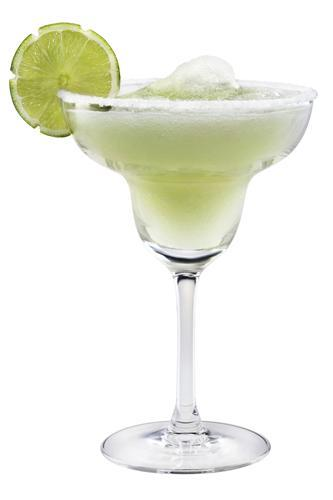
\includegraphics[height=6cm]{margarita}

\end{multicols}


\subsection*{Method}
Rim the edge of a cocktail glass with salt by coating the edge with lime juice and dipping into the salt.
Add the other ingredients to a cocktail shaker with a few cubes of ice.
Shake well for 10-15 seconds or until the outside of the shaker becomes frosted.
Strain into a cocktail glass and serve.

\section{Fitzgerald}

\subsection*{Ingredients}

\begin{multicols}{2}

\begin{tabular} { r | l}
    25ml & Lemon Juice \\
    15ml & Simple Syrup \\
    2 dashes & Angostura Bitter \\
    50ml & Dry Gin
\end{tabular}

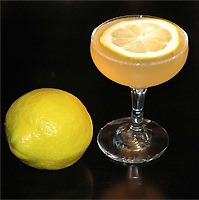
\includegraphics[height=6cm]{fitzgerald}

\end{multicols}


\subsection*{Method}
Add all ingredients to a cocktail shaker with ice and shake well.
Strain into a chilled cocktail glass. Garnish with a lemon wedge and serve.

\end{document}